
% ----------------------------------------------------------------------
%  Set the document class
% ----------------------------------------------------------------------
\documentclass[11pt,a4paper,twoside]{article}

% ----------------------------------------------------------------------
% Define external packages, language, margins, fonts and new commands
% ----------------------------------------------------------------------
%\input{preamble} 
\usepackage[utf8]{inputenc}   % <<<<< Linux
\usepackage[english]{babel} % <<<<< English
\usepackage{notoccite}
\usepackage[skip=0.5\baselineskip]{caption}
\hyphenation{GTKWave}
\usepackage{listings}
\usepackage[all]{nowidow}

%blind text
\usepackage{lipsum}

\usepackage{graphicx}
\graphicspath{{./}{../../figlib/}{../mat/}{../sim/}}
\def\FontLn{% 16 pt normal
  \usefont{T1}{phv}{m}{n}\fontsize{16pt}{16pt}\selectfont}
\def\FontLb{% 16 pt bold
  \usefont{T1}{phv}{b}{n}\fontsize{16pt}{16pt}\selectfont}
\def\FontMn{% 14 pt normal
  \usefont{T1}{phv}{m}{n}\fontsize{14pt}{14pt}\selectfont}
\def\FontMb{% 14 pt bold
  \usefont{T1}{phv}{b}{n}\fontsize{14pt}{14pt}\selectfont}
\def\FontSn{% 12 pt normal
  \usefont{T1}{phv}{m}{n}\fontsize{12pt}{12pt}\selectfont}

% Use Arial font as default
%
\renewcommand{\rmdefault}{phv}
\renewcommand{\sfdefault}{phv}
\usepackage{geometry}	
\geometry{verbose,tmargin=2.5cm,bmargin=2.5cm,lmargin=2.5cm,rmargin=2.5cm}

%\usepackage{setspace}
%\renewcommand{\baselinestretch}{1.5}

\usepackage[pdftex]{hyperref} % enhance documents that are to be
                              % output as HTML and PDF
\hypersetup{colorlinks,       % color text of links and anchors,
                              % eliminates borders around links
%            linkcolor=red,    % color for normal internal links
            linkcolor=black,  % color for normal internal links
            anchorcolor=black,% color for anchor text
%            citecolor=green,  % color for bibliographical citations
            citecolor=black,  % color for bibliographical citations
%            filecolor=magenta,% color for URLs which open local files
            filecolor=black,  % color for URLs which open local files
%            menucolor=red,    % color for Acrobat menu items
            menucolor=black,  % color for Acrobat menu items
%            pagecolor=red,    % color for links to other pages
            pagecolor=black,  % color for links to other pages
%            urlcolor=cyan,    % color for linked URLs
            urlcolor=black,   % color for linked URLs
	          bookmarks=true,         % create PDF bookmarks
	          bookmarksopen=false,    % don't expand bookmarks
	          bookmarksnumbered=true, % number bookmarks
	          pdftitle={report},
            pdfauthor={Andre C. Marta},
%            pdfsubject={Thesis Title},
%            pdfkeywords={Thesis Keywords},
            pdfstartview=FitV,
            pdfdisplaydoctitle=true}

\usepackage[numbers,sort&compress]{natbib} % <<<<< References in numbered list [1],[2],...
\usepackage{subcaption} 
\usepackage{mdframed}

%%%%%%%%%%%%%%%%%%%%%%%%%%%%%%%%%%%%%%%%%%%%%%%%%%%%%%%%%%%%%%%%%%%%%%%%
%     Begin Document                                                   %
%%%%%%%%%%%%%%%%%%%%%%%%%%%%%%%%%%%%%%%%%%%%%%%%%%%%%%%%%%%%%%%%%%%%%%%%


\begin{document}

% Set plain page style (no headers, footer with centered page number)
\pagestyle{plain}

% Set roman numbering (i,ii,...) before the start of chapters
%\pagenumbering{roman}

% ----------------------------------------------------------------------
%  Cover page
% ----------------------------------------------------------------------
%%%%%%%%%%%%%%%%%%%%%%%%%%%%%%%%%%%%%%%%%%%%%%%%%%%%%%%%%%%%%%%%%%%%%%%%
%                                                                      %
%                                      %
%                                                                      %
%%%%%%%%%%%%%%%%%%%%%%%%%%%%%%%%%%%%%%%%%%%%%%%%%%%%%%%%%%%%%%%%%%%%%%%%

\thispagestyle {empty}

% IST Logo - Signature A
% parameters: bb=llx lly urx ury (bounding box), width=h_length, height=v_length, angle=angle, scale=factor, clip=true/false, draft=true/false. 
\includegraphics[bb=9.5cm 11cm 0cm 0cm,scale=0.29]{IST_A_CMYK_POS}

\begin{center}
%
% Figure (Image or plot)
\vspace{1.0cm}
% height = 50 mm
%\includegraphics[height=50mm]{Figures/Airbus_A350.jpg}

% Title, author and degree
\vspace{1cm}
{\FontLb Circuit Theory and Electronics Fundamentals} \\ % <<<<< EDIT TITLE
\vspace{1cm}
{\FontLb T2} \\
\vspace{1cm}
{\FontSn Physics Engineering, Técnico, University of Lisbon} \\ % <<<<< EDIT COURSE
\vspace{1cm}
{\FontSn April 5, 2021} \\ % <<<<< EDIT DATE (corresponds to date of oral examination)
%
\end{center}



% ----------------------------------------------------------------------
% Dedication page (optional)
% ----------------------------------------------------------------------
%\input{dedication} 
%\cleardoublepage

% ----------------------------------------------------------------------
%  Acknowledgments (optional)
% ----------------------------------------------------------------------
%\input{acknowledgements}
%\cleardoublepage

% ----------------------------------------------------------------------
%  Abstract (both in English and Portuguese)
% ----------------------------------------------------------------------
%\input{resumo} 
%\cleardoublepage

%\input{abstract} 

% ----------------------------------------------------------------------
%  Table of contents, list of tables, list of figures and nomenclature
% ----------------------------------------------------------------------

% Table of contents
%
\tableofcontents

% List of tables
%\addcontentsline{toc}{section}{\listtablename}
%\listoftables
%\cleardoublepage 

% List of figures
%\addcontentsline{toc}{section}{\listfigurename}
%\listoffigures
%\cleardoublepage 

% Set arabic numbering (1,2,...) after preface
%
%\setcounter{page}{1}
%\pagenumbering{arabic}

% ----------------------------------------------------------------------
%  Body
% ----------------------------------------------------------------------

\section{Introduction}
\label{sec:introduction}
\paragraph{}
\par The objective of this laboratory assignment is to study a circuit that contains two current sources, two voltage sources and seven resistors. The circuit has a dependent voltage source $V_c$ and an independent one $V_a$. One of the current sources is dependent, $I_b$, and an independent one, $I_d$. 
\par A representation of the circuit made with \textit{LibreOffice Draw} can be seen in figure \ref{circuit}.

\begin{figure}[H]
    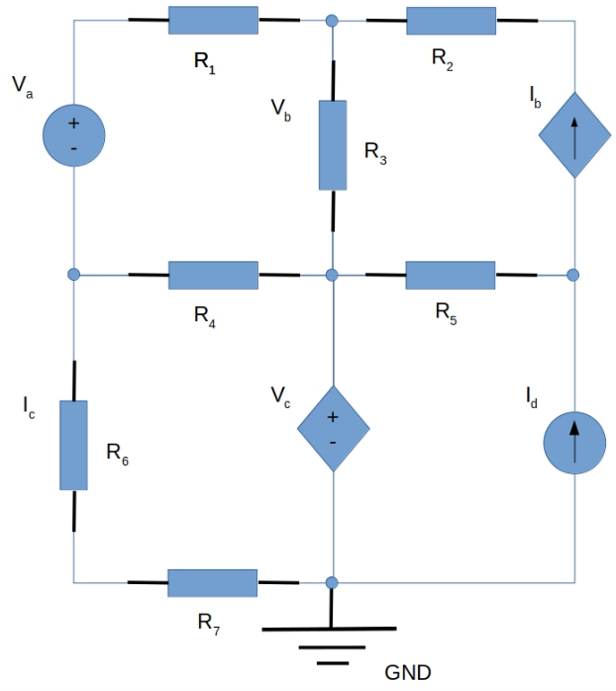
\includegraphics[width=0.4\linewidth]{Circuito.png}
    \centering
    \caption{Studied Circuit}
    \label{circuit}
\end{figure}

In Section~\ref{sec:analysis}, a theoretical analysis of the circuit is
presented. In Section~\ref{sec:simulation}, the circuit is analysed by
simulation, and the results are compared to the theoretical results obtained in
Section~\ref{sec:analysis}. The conclusions of this study are outlined in
Section~\ref{sec:conclusion}.



\section{Theoretical Analysis}
\label{sec:analysis}
\paragraph{}
\par In this section, the circuit shown in Figure \ref{circuit} is analysed
theoretically, using the mesh method and the nodes method. The known values can be seen in the following table.
\begin{table}[H]
    \centering
    \begin{tabular}{|c|c|}
    \hline
        $R_1$ & 1.02362892933kOhm \\ \hline 
        $R_2$ & 2.08640382129kOhm \\ \hline
        $R_3$ & 3.09996108706kOhm \\ \hline
        $R_4$ & 4.08183334334kOhm \\ \hline
        $R_5$ & 3.0416957579kOhm  \\ \hline
        $R_6$ & 2.04156679366kOhm \\ \hline
        $R_7$ & 1.04156790057kOhm \\ \hline
        $V_a$ & 5.17885996884V \\ \hline
        $I_d$ & 1.04908336809mA \\ \hline
        $K_b$ & 7.29571922963mS \\ \hline
        $K_c$ & 8.16840649221kOhm \\ \hline	
    \end{tabular}
    \caption{Known Data}
    \label{data}
\end{table}
\subsection{Mesh Method}
\paragraph{}
\par To fully understand this particular method, the concept of mesh needs to be clarified. A mesh is a loop that contains no other loops. Then, it is possible to determine, via Kirchhoff Voltage Law (KVL), the current in each mesh. With that information, using Ohm's Law, it is possible to determine every voltage in the circuit, knowing the resistances in the mesh. This method requires an attentive observer that can identify meshes, therefore, is not often used in automation processes.

\par Firstly, four meshes were indentified in the circuit. The equations were writen and the flow of the current was stipulated, as can be seen in figure \ref{mesh}. 

\begin{figure}[H]
    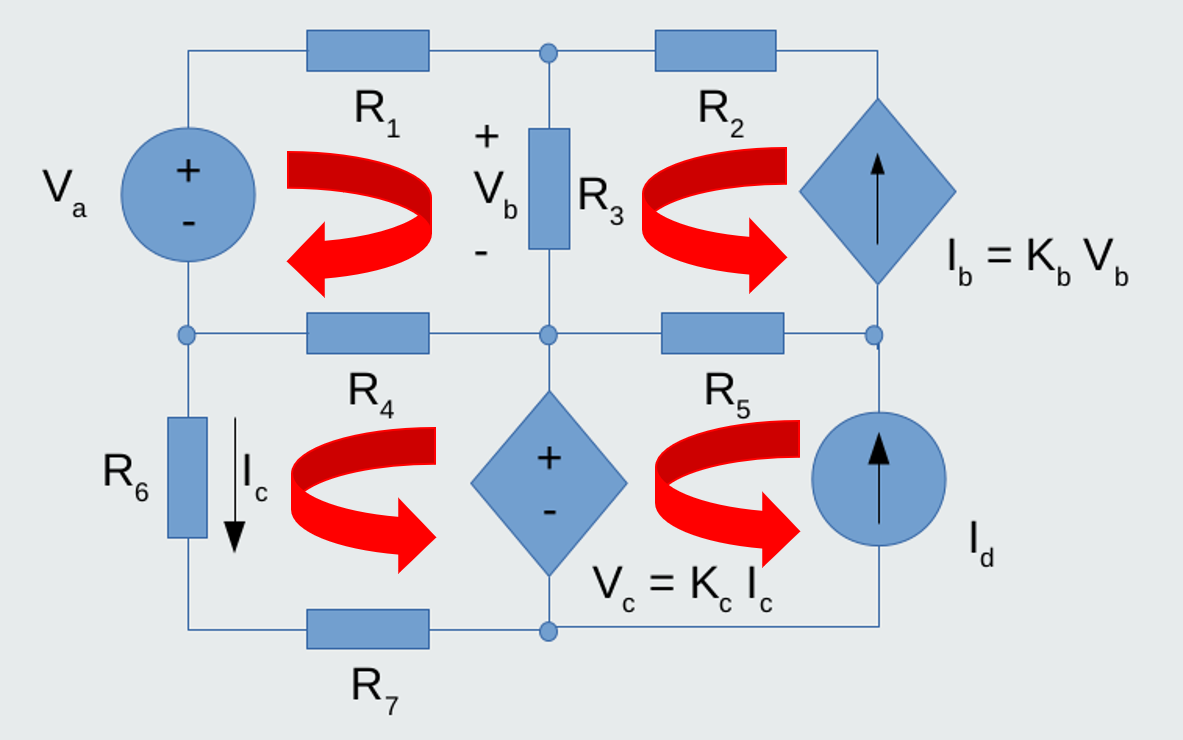
\includegraphics[width=0.5\linewidth]{Mesh.png}
    \centering
    \caption{Mesh Method applied to the circuit}
    \label{mesh}
\end{figure}

\par Simplifying the mesh method, the following system of equations \ref{system mesh} was writen. 
$$
\begin{cases} 
	V_a = R_{1}I_{a}+R_{3}(I_{a}+I_{b})+R_{4}(I_{a}+I_{c}) \\ 
	V_b = \frac{I_{b}}{K_{b}} = R_{3}(I_{a}+I_{b}) \\ 
	V_c = K_{c}I_{c} = R_{4}(I_{a}+I_{c})+R_{6}I_{c}+R_{7}I_{c}
\label{system mesh}
\end{cases}
$$


\par It was transformed into the following system \ref{matrix} and solved using the software \textit{Octave}. 

\begin{equation}
	\begin{bmatrix}
		R_1+R_3+R_4 & R_3 & R_4 & 0 \\
		R_4 & 0 & -K_c+R_4+R_6+R_7 & 0 \\
		R_3 & R_3-\frac{1}{K_b} & 0 & 0 \\
		0 & 0 & 0 & 1
	\end{bmatrix}
	\begin{bmatrix}
		I_a     \\
		I_b     \\
		I_c \\
		I_d     \\
	\end{bmatrix}
    =
	\begin{bmatrix}
		V_a     \\
		0     \\
		0  \\
		0     \\
	\end{bmatrix}
	\label{matrix}
\end{equation}

\par Therefore, the values for the voltage and current sources were determined and can be seen in the following table \ref{results mesh}, being the unit for current mA and the unit for voltage V. 

\begin{table}[H]
    \centering
    \begin{tabular}{|c|c|}
    \hline
        $I_a$ & 2.401364132117077e-01 \\ \hline 
        $I_b$ & 2.512453816512571e-01 \\ \hline
        $I_c$ & 9.768380052260230e-01 \\ \hline
        $I_d$ & 1.049083368090000e+00 \\ \hline
        $V_a$ & 5.178859968840000 \\ \hline
        $V_b$ & 3.443736987998083e-02 \\ \hline
        $V_c$ & 7.979209903725712\\ \hline
    \end{tabular}
    \caption{Table of results for the mesh method}
    \label{results mesh}
\end{table}

\subsection{Node Method}
\paragraph{}
\par Nodes are any regions between any two elements of the circuit. With Kirchhoff Current Law (KCL) it is possible to determine any nodal voltage. The KCL cannot be used in nodes that are connected to a voltage source. This means those nodes must have relations with the source, making it possible to solve the system. In opposition to the mesh method, this method is easy to automate due to its methodical approach, being possible to extract values in a simulation very easily.
The first approach is to name every node so it is possible to start the analysis.


\par First, the nodes were represented in the circuit as can be seen in figure \ref{circuitlt}. The software used to represent the circuit and to provide another simulation to confirm the one explained on \ref{sec:simulation} was \textit{LTSpice}.

\begin{figure}[H]
    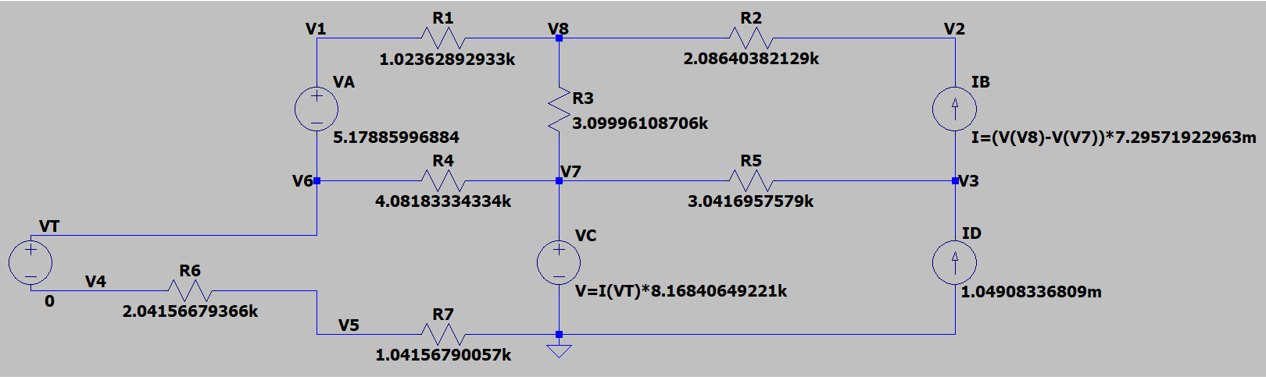
\includegraphics[width=0.8\linewidth]{CircuitLTSpice.png}
    \centering
    \caption{Circuit represented through \textit{LTSpice}}
    \label{circuitlt}
\end{figure}


\par Then, the equations for the nodes method were writen according to the numeration visible in the circuit above. The voltage source $V_T$ was created to help in the simulation analysis, the reason behind it will be explained later.
$$
\begin{cases} 
	V_1 - V_6 = V_a \\ 
	\frac{V_2 - V_8}{R_2} - K_b*(V_8 - V_7) = 0 \\
	-I_d + \frac{V_3 - V_7}{R_5} + K_{b}(V_8 - V_7) = 0 \\ 
	\frac{V_5 - V_6}{R_6} + \frac{V_5}{R_7} = 0 \\
	\frac{V_8 - V_1}{R_1} + \frac{V_8 - V_2}{R_2} - \frac{V_8 - V_7}{R_3}  = 0 \\
	\frac{V_6 - V_7}{R_4} + \frac{V_6 - V_5}{R_6} - \frac{V_1 - V_8}{R_1}  = 0 \\
	V_7 = -K_c \frac{V_5 - V_6}{R_6}
\label{system nodes}
\end{cases}
$$
\par The equations above were transformed into the following system \ref{matrixn} so that \textit{Octave} could solve it.
\begin{equation}
	\begin{bmatrix}
		1 & 0 & 0 & 0 &-1 & 0 & 0 \\
		0 & \frac{1}{R_2} & 0 & 0 & 0 & K_b & \frac{-1}{R_2}-K_b \\
		0 & 0 & \frac{1}{R_5} & 0 & 0 & \frac{-1}{R_5}-K_b & K_b \\
		0 & 0 & 0 & \frac{1}{R_6}+\frac{1}{R_7} & \frac{-1}{R_6} & 0 & 0 \\
		\frac{-1}{R_1} & \frac{-1}{R_2} & 0 & 0 & 0 & \frac{-1}{R_3} & \frac{1}{R_1}+\frac{1}{R_2}+\frac{1}{R_3} \\
		\frac{1}{R_1} & 0 & 0 & \frac{-1}{R_6} & \frac{1}{R_4}+\frac{1}{R_6} & \frac{-1}{R_4} & \frac{-1}{R_1} \\
		0 & 0 & 0 & \frac{K_c}{R_6} & \frac{-K_c}{R_6} & 1 & 0]
	\end{bmatrix}
	\begin{bmatrix}
		V_1     \\
		V_2     \\
		V_3  \\
		V_5  \\
		V_6   \\
		V_7   \\ 
		V_8     \\
	\end{bmatrix}
    =
	\begin{bmatrix}
		V_a     \\
		0     \\
		I_d  \\
		0     \\
		0     \\
		0     \\
		0     \\
	\end{bmatrix}
	\label{matrixn}
\end{equation}

\par Hence, the values for the current sources and the voltage in each point $V_1$ to $V_8$ were calculated and can be seen in the table below, again being the unit for current mA and the unit for voltage V. $V_4$ is only in the circuit for simulation purposes, with voltage equal to $V_6$, $V_4$ is supressed in the analysis.

\begin{table}[H]
    \centering
    \begin{tabular}{|c|c|}
    \hline
        $V_1$ & 8.190583113394776e+00\\ \hline
        $V_2$ & 7.420573209487090e+00\\ \hline
        $V_3$ & 1.193441434568911e+01\\ \hline
        $V_5$ & 1.017443110300255e+00\\ \hline
        $V_6$ & 3.011723144554777e+00\\ \hline
        $V_7$ & 7.979209903725710e+00\\ \hline
        $V_8$ & 7.944772533845730e+00\\ \hline
        $I_a$ & 2.401364132117075e-01\\ \hline 
        $I_b$ & 2.512453816512545e-01\\ \hline
        $I_c$ & 9.768380052260227e-01\\ \hline
        $I_d$ & 1.049083368090000e+00\\ \hline
    \end{tabular}
    \caption{Table of results for the node method}
    \label{results node}
\end{table}

\par Using
\begin{equation}
	V_b=\frac{I_b}{K_b}
\label{Vb}
\end{equation}
and
\begin{equation}
	V_c=K_{c}I_{c}
\end{equation}
one can get the following results:
\begin{table}[H]
    \centering
    \begin{tabular}{|c|c|}
    \hline
        $V_a$ & 5.178859968840000\\ \hline
        $V_b$ & 3.443736987998047e-02\\ \hline
        $V_c$ & 7.979209903725709\\ \hline
    \end{tabular}
    \caption{Values of $V_a$, $V_b$ and $V_c$}
\end{table}

\par It is evident that the two methods return values with notorious resemblance.

\par The simulation, explained on the next section, will be compared with the two theoretichal analysis in order to identify any incompability with the theory, allowing further discussion.


\section{Simulation Analysis}
\label{sec:simulation}

\subsection{Operating Point Analysis}

Table~\ref{tab:op} shows the simulated operating point results for the circuit
under analysis. Compared to the theoretical analysis results, one notices the
following differences: describe and explain the differences.

\begin{table}[h]
  \centering
  \begin{tabular}{|l|r|}
    \hline    
    {\bf Name} & {\bf Value [A or V]} \\ \hline
    @cb[i] & 0.000000e+00\\ \hline
@ce[i] & 0.000000e+00\\ \hline
@q1[ib] & 7.022567e-05\\ \hline
@q1[ic] & 1.404513e-02\\ \hline
@q1[ie] & -1.41154e-02\\ \hline
@q1[is] & 5.765392e-12\\ \hline
@rc[i] & 1.411536e-02\\ \hline
@re[i] & 1.411536e-02\\ \hline
@rf[i] & 7.022567e-05\\ \hline
@rs[i] & 0.000000e+00\\ \hline
v(1) & 0.000000e+00\\ \hline
v(2) & 0.000000e+00\\ \hline
base & 2.254108e+00\\ \hline
coll & 5.765392e+00\\ \hline
emit & 1.411536e+00\\ \hline
vcc & 1.000000e+01\\ \hline

  \end{tabular}
  \caption{Operating point. A variable preceded by @ is of type {\em current}
    and expressed in Ampere; other variables are of type {\it voltage} and expressed in
    Volt.}
  \label{tab:op}
\end{table}

\lipsum[1-1]


\subsection{Transient Analysis}

Figure~\ref{fig:trans} shows the simulated transient analysis results for the
circuit under analysis. Compared to the theoretical analysis results, one
notices the following differences: describe and explain the differences.

\begin{figure}[h] \centering
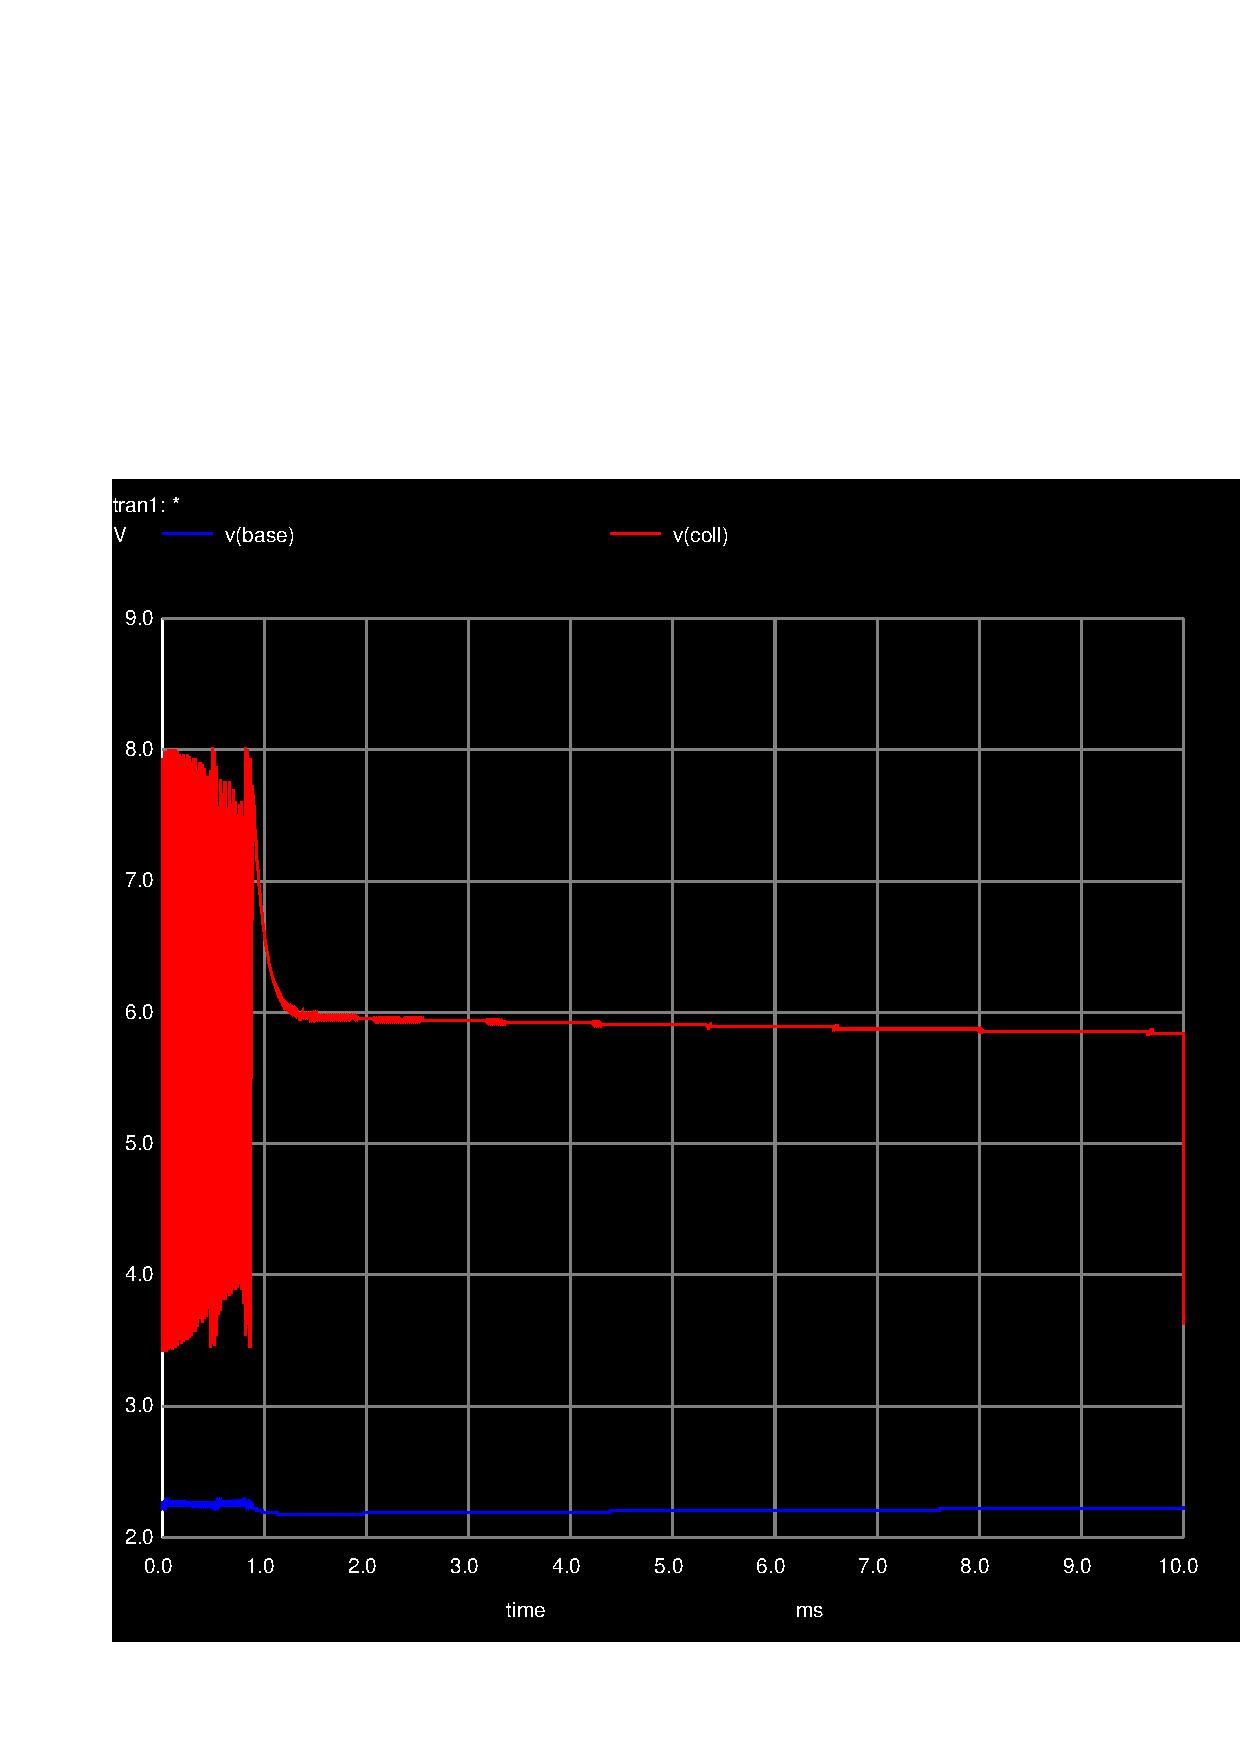
\includegraphics[width=0.6\linewidth]{trans.pdf}
\caption{Transient output voltage}
\label{fig:trans}
\end{figure}

\lipsum[1-1]



\subsection{Frequency Analysis}

\subsubsection{Magnitude Response}

Figure~\ref{fig:acm} shows the magnitude of the frequency response for the
circuit under analysis. Compared to the theoretical analysis results, one
notices the following differences: describe and explain the differences.

\begin{figure}[h] \centering
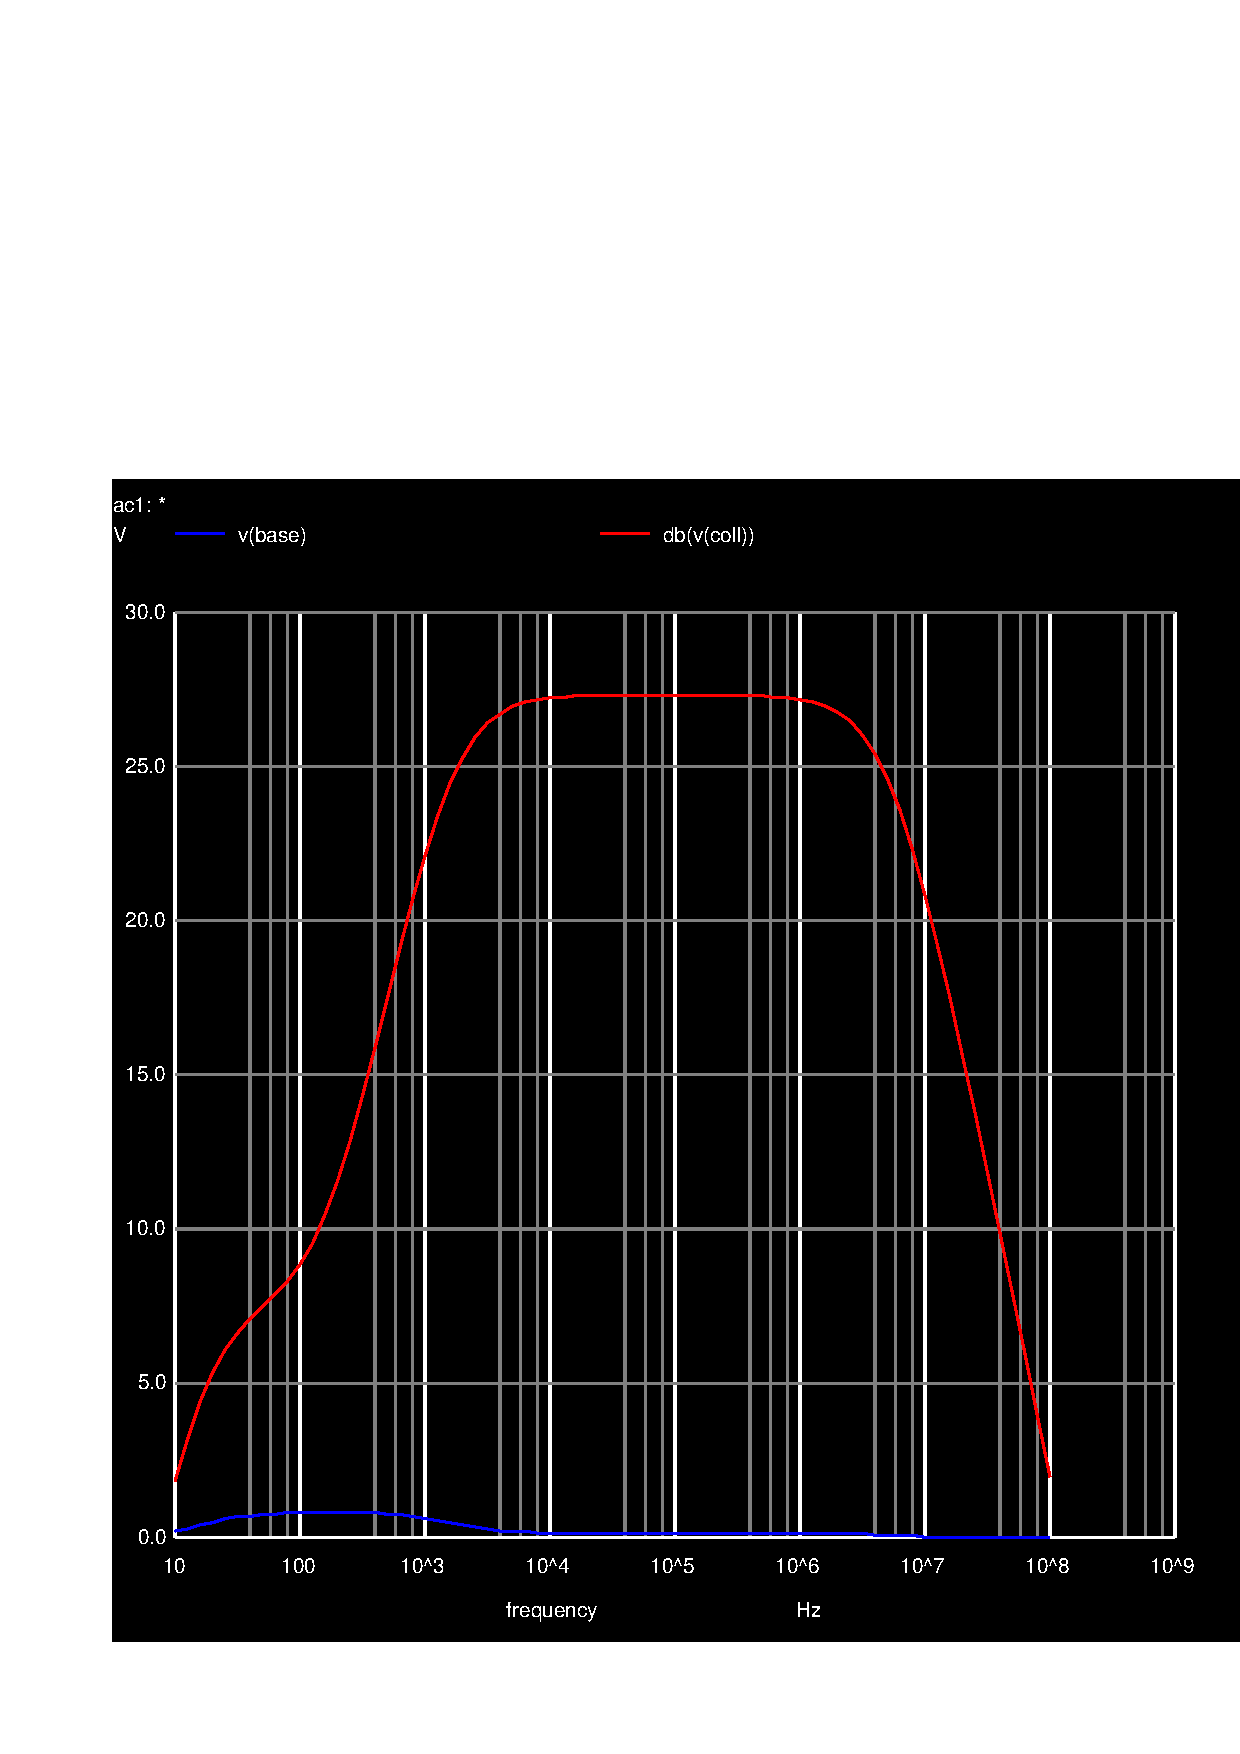
\includegraphics[width=0.6\linewidth]{acm.pdf}
\caption{Magnitude response}
\label{fig:acm}
\end{figure}

\lipsum[1-1]

\subsubsection{Phase Response}

Figure~\ref{fig:acp} shows the magnitude of the frequency response for the
circuit under analysis. Compared to the theoretical analysis results, one
notices the following differences: describe and explain the differences.

\begin{figure}[h] \centering
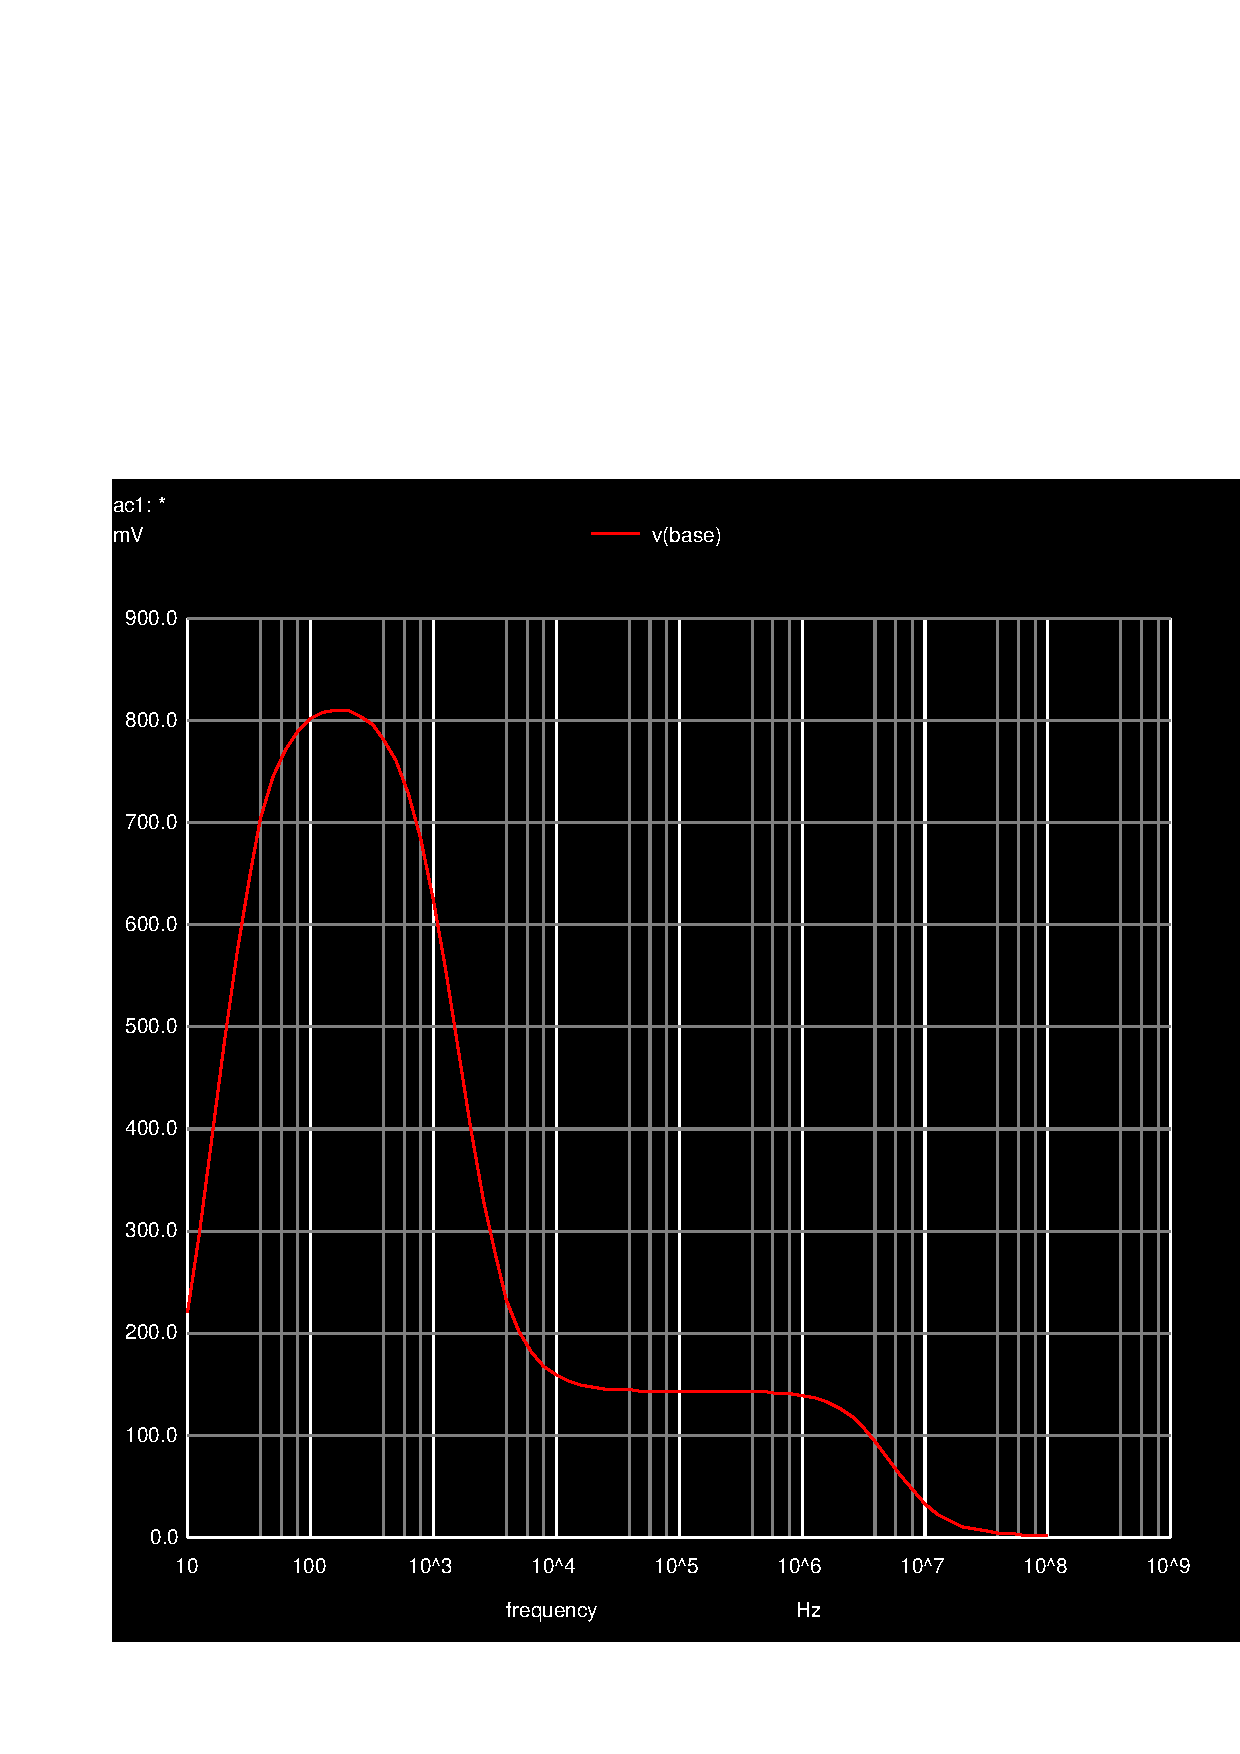
\includegraphics[width=0.6\linewidth]{acp.pdf}
\caption{Phase response}
\label{fig:acp}
\end{figure}

\lipsum[1-1]

\subsubsection{Input Impedance}

Figure~\ref{fig:zim} shows the magnitude of the frequency response for the
circuit under analysis. Compared to the theoretical analysis results, one
notices the following differences: describe and explain the differences.

\begin{figure}[h] \centering
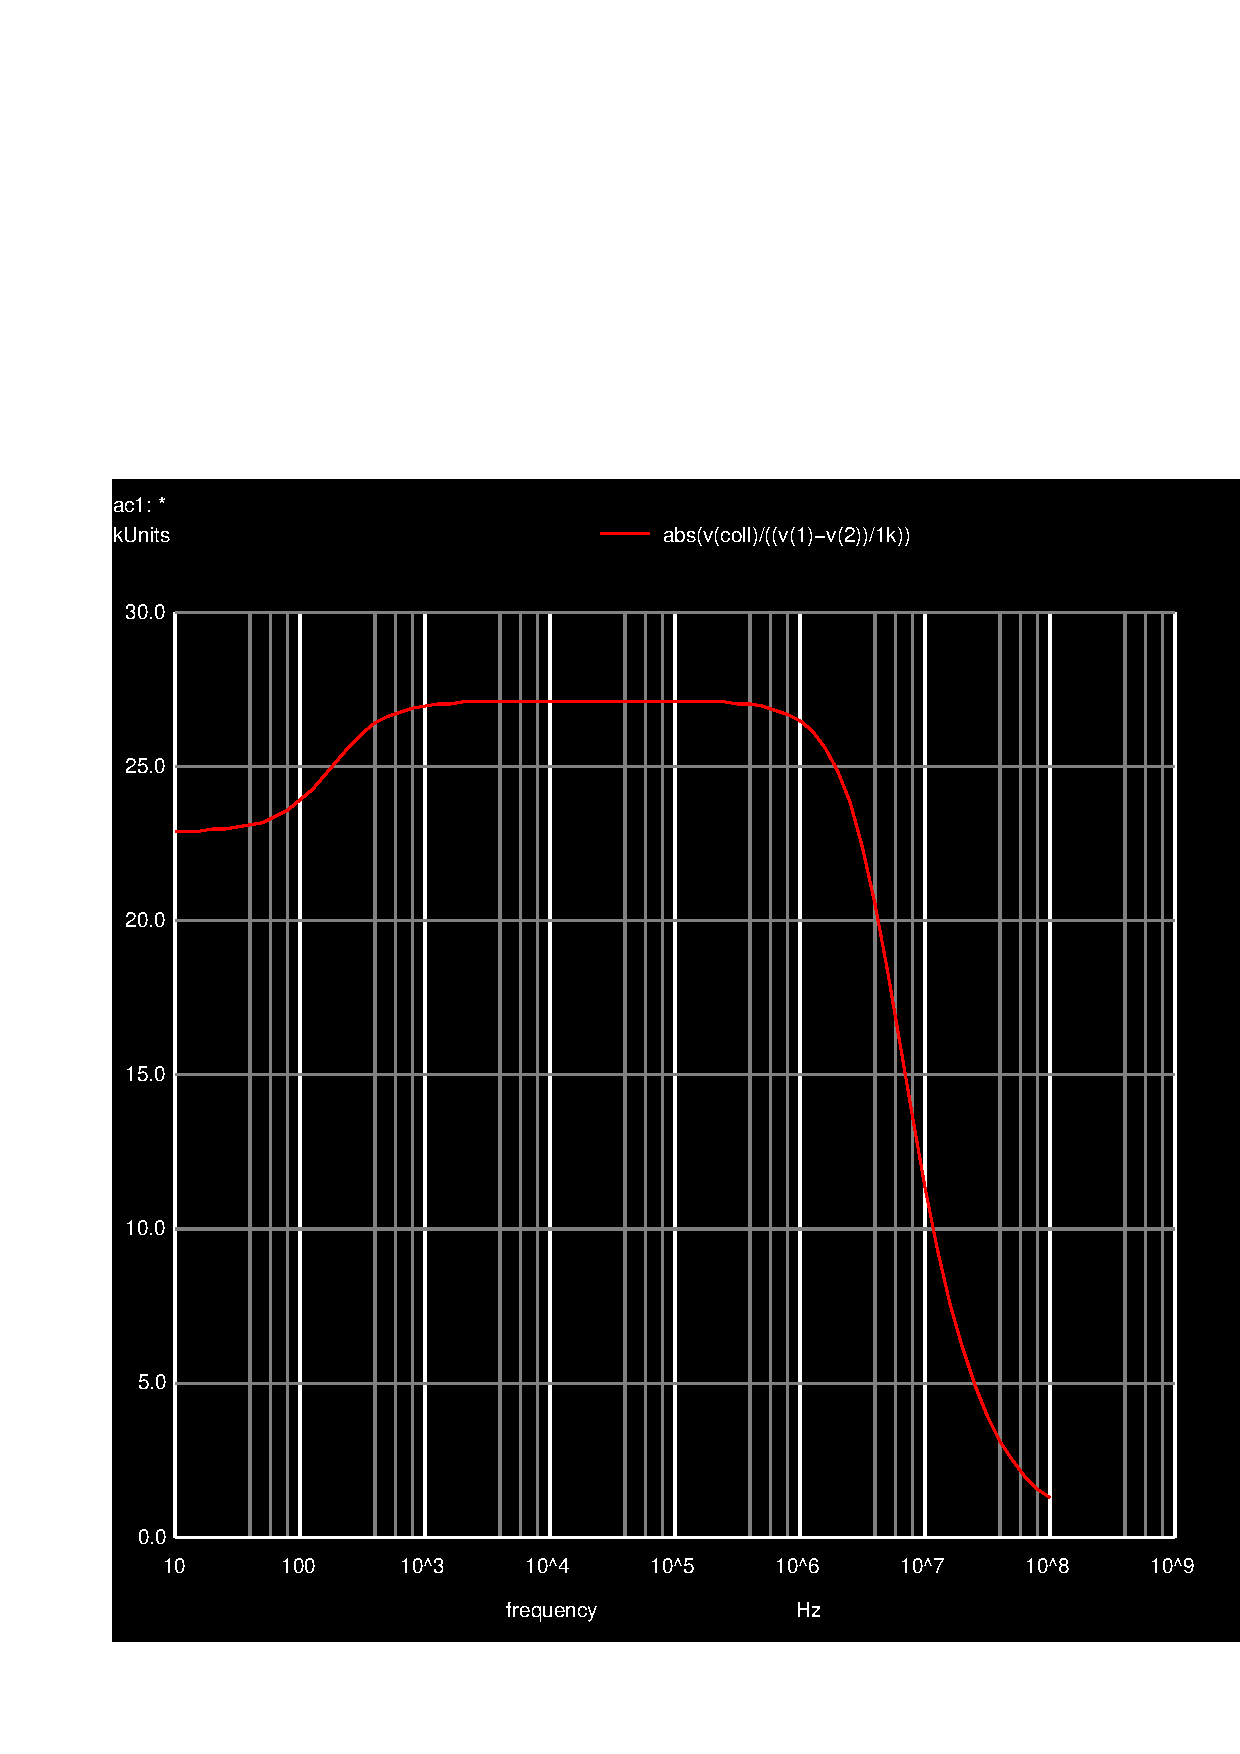
\includegraphics[width=0.6\linewidth]{zim.pdf}
\caption{Input impedance}
\label{fig:zim}
\end{figure}

\lipsum[1-1]





\section{Conclusion}
\label{sec:conclusion}

In this laboratory assignment the objective of analysing an RC circuit has been
achieved. Static, time and frequency analyses have been performed both
theoretically using the Octave maths tool and by circuit simulation using the
Ngspice tool. The simulation results matched the theoretical results
precisely. The reason for this perfect match is the fact that this is a
straightforward circuit containing only linear components, so the theoretical
and simulation models cannot differ. For more complex components, the
theoretical and simulation models could differ but this is not the case in this
work.

\lipsum[1-1]

%\cleardoublepage

% ----------------------------------------------------------------------
%  Bibliography
% ----------------------------------------------------------------------
%\addcontentsline{toc}{section}{\bibname}
%\bibliographystyle{abbrvunsrtnat} % <<<<< SELECT IF USING REFERENCES BY NUMBER (CITATION ORDER)
%\bibliography{../../../BIBfile.bib}

% ----------------------------------------------------------------------
\end{document}
% ----------------------------------------------------------------------
